\documentclass[10pt]{beamer}

\usetheme{metropolis}
\usepackage{appendixnumberbeamer}
\usepackage{booktabs}
\usepackage[scale=2]{ccicons}
\usepackage{pgfplots}
\usepgfplotslibrary{dateplot}
\usepackage[T1]{fontenc}
\usepackage{graphicx}

\usepackage{tikz}
\usetikzlibrary{positioning,arrows,shapes}
\pgfplotsset{compat=1.18}

\metroset{titleformat=smallcaps,numbering=fraction}

\title{Policy Conflicts and Strategies in the Policy-Making Process}
\subtitle{POSC 315: Introduction to Public Policy}
\date{\today}
\author{David P. Adams, Ph.D.}
\institute{California State University, Fullerton}

\begin{document}

\maketitle

\begin{frame}{Table of contents}
  \setbeamertemplate{section in toc}[sections numbered]
  \tableofcontents[hideallsubsections]
\end{frame}

\begin{frame}
    \frametitle{Learning Objectives}
    \begin{itemize}
        \item Understand the \alert{sources} of policy conflict
        \item Explore \alert{strategies} to manage or resolve policy conflicts
        \item Reflect on how conflict can serve as both a \alert{challenge} and an \alert{opportunity}
        \item Develop a foundation for applying these concepts to \alert{real-world policy issues}
    \end{itemize}
    
    \begin{figure}
        \centering
        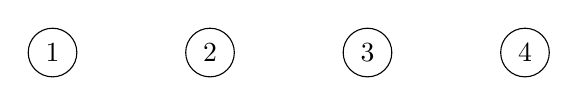
\begin{tikzpicture}
            \node[draw, circle] at (0,0) {1};
            \node[draw, circle] at (2,0) {2};
            \node[draw, circle] at (4,0) {3};
            \node[draw, circle] at (6,0) {4};
        \end{tikzpicture}
        \caption{Learning Objectives}
    \end{figure}
\end{frame}

\begin{frame}
    \frametitle{What is Policy Conflict?}
    \begin{itemize}
        \item \textbf{Definition:} A situation where stakeholders have \alert{opposing interests, goals, or values}
        \item \textbf{Key Elements:}
            \begin{itemize}
                \item \textbf{Competing Interests:} Economic vs. environmental priorities
                \item \textbf{Value Clashes:} Individual rights vs. collective welfare
                \item \textbf{Limited Resources:} Funding, time, or personnel
            \end{itemize}
    \end{itemize}
    
    \begin{figure}
        \centering
        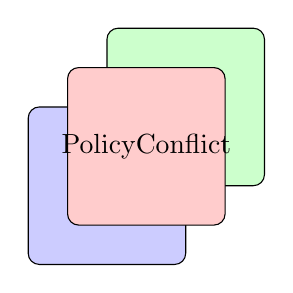
\begin{tikzpicture}
            \draw[fill=blue!20, rounded corners] (0,0) rectangle (2,2);
            \draw[fill=green!20, rounded corners] (1,1) rectangle (3,3);
            \draw[fill=red!20, rounded corners] (0.5,0.5) rectangle (2.5,2.5);
            \node at (1.5,1.5) {Policy\\Conflict};
        \end{tikzpicture}
        \caption{Elements of Policy Conflict}
    \end{figure}
\end{frame}

    \begin{figure}
        \centering
        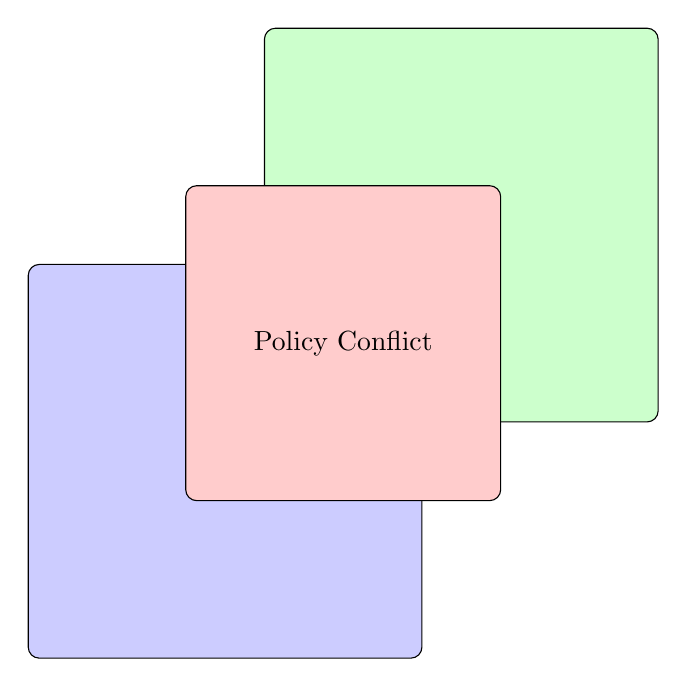
\begin{tikzpicture}
            \draw[fill=blue!20, rounded corners] (0,0) rectangle (5,5);
            \draw[fill=green!20, rounded corners] (3,3) rectangle (8,8);
            \draw[fill=red!20, rounded corners] (2,2) rectangle (6,6);
            \node at (4,4) {Policy Conflict};
        \end{tikzpicture}
        \caption{Elements of Policy Conflict}
    \end{figure}
    \end{frame}
    
    \begin{frame}
    \frametitle{Common Sources of Conflict}
    \begin{enumerate}
        \item \textbf{Differing Stakeholder Interests:}
            \begin{itemize}
                \item Example: Businesses prioritize profits; activists prioritize sustainability.
            \end{itemize}
        \item \textbf{Ideological Differences:}
            \begin{itemize}
                \item Example: Debates over government intervention in healthcare.
            \end{itemize}
        \item \textbf{Resource Limitations:}
            \begin{itemize}
                \item Limited budgets often spark competition for allocation.
            \end{itemize}
        \item \textbf{Regulatory Constraints:}
            \begin{itemize}
                \item Federal vs. state jurisdiction conflicts.
            \end{itemize}
    \end{enumerate}
    
    \begin{figure}
        \centering
        \begin{tikzpicture}
            \node[draw, circle, minimum size=2cm] (interests) {\includegraphics[width=1.5cm]{briefcase.png}};
            \node[draw, circle, minimum size=2cm, right of=interests, xshift=3cm] (ideology) {\includegraphics[width=1.5cm]{debate.png}};
            \node[draw, circle, minimum size=2cm, right of=ideology, xshift=3cm] (resources) {\includegraphics[width=1.5cm]{money-bag.png}};
            \node[draw, circle, minimum size=2cm, right of=resources, xshift=3cm] (regulations) {\includegraphics[width=1.5cm]{gavel.png}};
        \end{tikzpicture}
        \caption{Sources of Policy Conflict}
    \end{figure}
    \end{frame}
    
    \begin{frame}
    \frametitle{Stakeholder Interest Conflicts}
    \begin{columns}[T,onlytextwidth]
        \column{0.5\textwidth}
        \begin{block}{Environmental Policy Example}
            \begin{itemize}
                \item \textbf{Conflict:} Economic development vs. conservation.
                \item \textbf{Stakeholders:} Industry, environmental groups, local communities.
            \end{itemize}
        \end{block}
        \column{0.5\textwidth}
        \begin{block}{Social Policy Example}
            \begin{itemize}
                \item \textbf{Conflict:} Equity vs. efficiency in welfare programs.
                \item \textbf{Stakeholders:} Taxpayers, beneficiaries, policymakers.
            \end{itemize}
        \end{block}
    \end{columns}
    
    \begin{figure}
        \centering
        \begin{tikzpicture}
            \node[draw, circle, minimum size=2cm] (factory) {\includegraphics[width=1.5cm]{images/factory.png}};
            \node[draw, circle, minimum size=2cm, right of=factory, xshift=3cm] (forest) {\includegraphics[width=1.5cm]{forest.png}};
        \end{tikzpicture}
        \caption{Stakeholder Interest Conflicts}
    \end{figure}
    \end{frame}
    

    \begin{frame}
        \frametitle{Ideological Clashes in Policy}
        \begin{itemize}
            \item Examples of Ideological Conflicts:
                \begin{enumerate}
                    \item \textbf{Healthcare Reform:} Individual responsibility vs. collective welfare.
                    \item \textbf{Tax Policies:} Redistribution vs. growth-oriented strategies.
                \end{enumerate}
            \item \textbf{Impact:}
                \begin{itemize}
                    \item Polarized debates slow policymaking processes.
                \end{itemize}
        \end{itemize}
        
        \begin{figure}
            \centering
            \begin{tikzpicture}
                \begin{axis}[
                    width=0.9\textwidth,
                    height=6cm,
                    mbarplot,
                    xlabel={Year},
                    ylabel={Ideological Divide},
                    xtick={2010, 2012, 2014, 2016, 2018, 2020},
                    legend pos=north west
                ]
                
                \addplot plot coordinates {(2010, 65) (2012, 70) (2014, 75) (2016, 80) (2018, 85) (2020, 90)};
                \addplot plot coordinates {(2010, 60) (2012, 65) (2014, 70) (2016, 75) (2018, 80) (2020, 85)};
                \legend{House, Senate}
                \end{axis}
            \end{tikzpicture}
            \caption{Ideological Divide in U.S. Congress Over Time}
        \end{figure}
        \end{frame}

      
            

            \begin{frame}
                \frametitle{Bureaucratic and Regulatory Barriers}
                \begin{itemize}
                    \item \textbf{Definition:} Conflicts arising from overlapping or restrictive regulations.
                    \item Example:
                        \begin{itemize}
                            \item Federal vs. state laws on marijuana legalization.
                        \end{itemize}
                    \item \textbf{Impact on Policymaking:}
                        \begin{itemize}
                            \item Delayed implementation.
                            \item Increased litigation costs.
                        \end{itemize}
                \end{itemize}

                \begin{frame}
                    \frametitle{Stakeholder Interest Conflicts}
                    \begin{columns}[T,onlytextwidth]
                        \column{0.5\textwidth}
                        \begin{block}{Environmental Policy Example}
                            \begin{itemize}
                                \item \textbf{Conflict:} Economic development vs. conservation.
                                \item \textbf{Stakeholders:} Industry, environmental groups, local communities.
                            \end{itemize}
                        \end{block}
                        \column{0.5\textwidth}
                        \begin{block}{Social Policy Example}
                            \begin{itemize}
                                \item \textbf{Conflict:} Equity vs. efficiency in welfare programs.
                                \item \textbf{Stakeholders:} Taxpayers, beneficiaries, policymakers.
                            \end{itemize}
                        \end{block}
                    \end{columns}
                    
                    \vspace{0.5cm}
                    
                    \begin{figure}
                        \centering
                        \resizebox{0.8\textwidth}{!}{
                            \begin{tikzpicture}
                                \node[draw, circle, minimum size=2cm] (factory) {\includegraphics[width=1.5cm]{factory.png}};
                                \node[draw, circle, minimum size=2cm, right=3cm of factory] (forest) {\includegraphics[width=1.5cm]{forest.png}};
                            \end{tikzpicture}
                        }
                        \caption{\scriptsize Stakeholder Interest Conflicts}
                    \end{figure}
                \end{frame}
                
                \begin{frame}
                    \frametitle{Ideological Clashes in Policy}
                    \begin{itemize}
                        \item Examples of Ideological Conflicts:
                            \begin{enumerate}
                                \item \textbf{Healthcare Reform:} Individual responsibility vs. collective welfare.
                                \item \textbf{Tax Policies:} Redistribution vs. growth-oriented strategies.
                            \end{enumerate}
                        \item \textbf{Impact:}
                            \begin{itemize}
                                \item Polarized debates slow policymaking processes.
                            \end{itemize}
                    \end{itemize}
                    
                    \begin{figure}
                        \centering
                        \resizebox{0.9\textwidth}{!}{
                            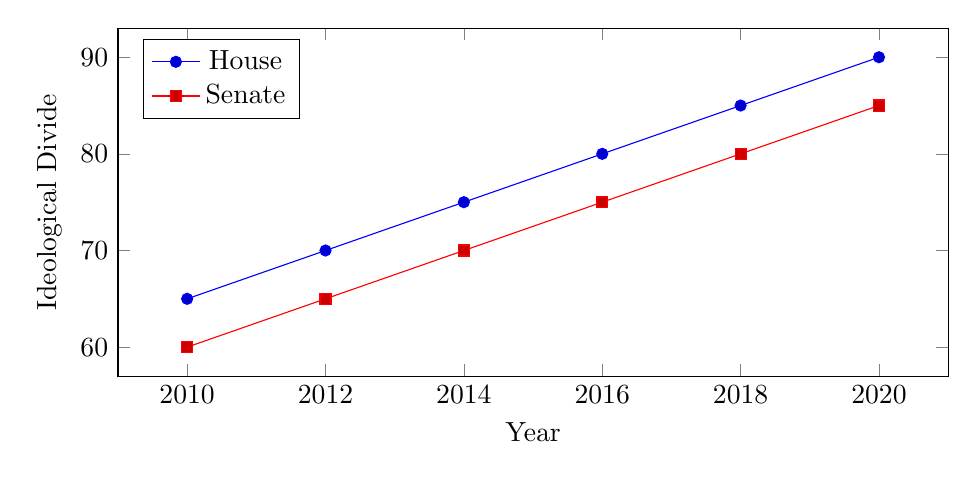
\begin{tikzpicture}
                                \begin{axis}[
                                    width=1.0\textwidth,
                                    height=6cm,
                                    xlabel={Year},
                                    ylabel={Ideological Divide},
                                    xtick={2010, 2012, 2014, 2016, 2018, 2020},
                                    xticklabels={2010, 2012, 2014, 2016, 2018, 2020},
                                    legend pos=north west
                                ]
                                \addplot plot coordinates {(2010, 65) (2012, 70) (2014, 75) (2016, 80) (2018, 85) (2020, 90)};
                                \addplot plot coordinates {(2010, 60) (2012, 65) (2014, 70) (2016, 75) (2018, 80) (2020, 85)};
                                \legend{House, Senate}
                                \end{axis}
                            \end{tikzpicture}
                        }
                        \caption{\scriptsize Ideological Divide in U.S. Congress Over Time}
                    \end{figure}
                \end{frame}
                
                \begin{frame}
                    \frametitle{Limited Resources as a Conflict Source}
                    \begin{itemize}
                        \item \textbf{Definition:} Insufficient resources create competition among stakeholders.
                        \item Examples:
                            \begin{enumerate}
                                \item \textbf{Infrastructure Funding:} Which projects get priority?
                                \item \textbf{Disaster Relief Allocation:} Balancing urgency and equity.
                            \end{enumerate}
                        \item \textbf{Outcome:} Resource constraints often lead to incremental decisions.
                    \end{itemize}
                    
                    \begin{figure}
                        \centering
                        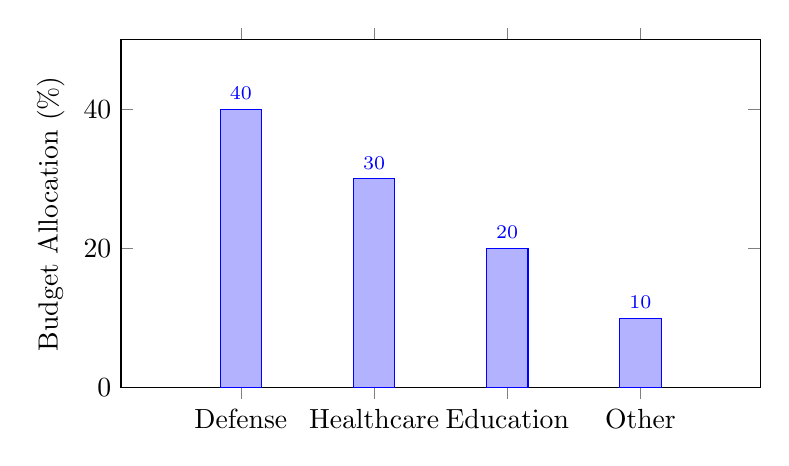
\begin{tikzpicture}
                            \begin{axis}[
                                ybar,
                                width=0.8\textwidth,
                                height=6cm,
                                bar width=15pt,
                                ylabel={Budget Allocation (\%)},
                                symbolic x coords={Defense, Healthcare, Education, Other},
                                xtick=data,
                                nodes near coords,
                                ymin=0,
                                ymax=50,
                                enlarge x limits=0.3,
                                every node near coord/.append style={font=\scriptsize}
                            ]
                                \addplot coordinates {(Defense, 40) (Healthcare, 30) (Education, 20) (Other, 10)};
                            \end{axis}
                        \end{tikzpicture}
                        \caption{\scriptsize Government Budget Allocation}
                    \end{figure}
                \end{frame}
                
                \begin{frame}
                    \frametitle{Bureaucratic and Regulatory Barriers}
                    \begin{itemize}
                        \item \textbf{Definition:} Conflicts arising from overlapping or restrictive regulations.
                        \item Example:
                            \begin{itemize}
                                \item Federal vs. state laws on marijuana legalization.
                            \end{itemize}
                        \item \textbf{Impact on Policymaking:}
                            \begin{itemize}
                                \item Delayed implementation.
                                \item Increased litigation costs.
                            \end{itemize}
                    \end{itemize}
                    
                    \begin{figure}
                        \centering
                        \resizebox{0.8\textwidth}{!}{
                            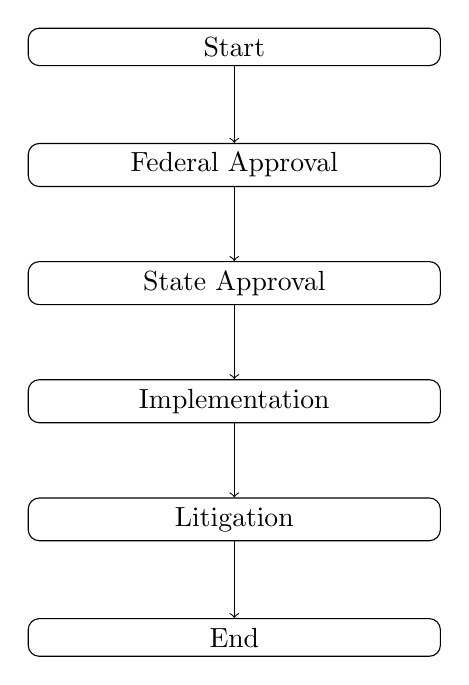
\begin{tikzpicture}[node distance=1.5cm]
                                \node[draw, rounded corners, text width=5cm, align=center] (start) {Start};
                                \node[draw, rounded corners, below of=start, text width=5cm, align=center] (federal) {Federal Approval};
                                \node[draw, rounded corners, below of=federal, text width=5cm, align=center] (state) {State Approval};
                                \node[draw, rounded corners, below of=state, text width=5cm, align=center] (implementation) {Implementation};
                                \node[draw, rounded corners, below of=implementation, text width=5cm, align=center] (litigation) {Litigation};
                                \node[draw, rounded corners, below of=litigation, text width=5cm, align=center] (end) {End};
                                
                                \draw[->] (start) -- (federal);
                                \draw[->] (federal) -- (state);
                                \draw[->] (state) -- (implementation);
                                \draw[->] (implementation) -- (litigation);
                                \draw[->] (litigation) -- (end);
                            \end{tikzpicture}
                        }
                        \caption{\scriptsize Regulatory Process Complexity}
                    \end{figure}
                \end{frame}
                

                \begin{frame}
                    \frametitle{Managing Policy Conflicts}
                    \begin{itemize}
                        \item \textbf{Key Strategies:}
                            \begin{enumerate}
                                \item \textbf{Negotiation:} Direct discussions for compromise.
                                \item \textbf{Mediation:} Third-party facilitation.
                                \item \textbf{Collaboration:} Joint decision-making.
                                \item \textbf{Litigation:} Resolving disputes through courts.
                            \end{enumerate}
                        \item \textbf{Importance:} Effective management ensures progress and stakeholder satisfaction.
                    \end{itemize}
                    
                    \begin{figure}
                        \centering
                        \begin{tikzpicture}
                            \node[draw, circle, minimum size=2cm] (negotiation) {\includegraphics[width=1.5cm]{handshake.png}};
                            \node[draw, circle, minimum size=2cm, right of=negotiation, xshift=3cm] (mediation) {\includegraphics[width=1.5cm]{mediator.png}};
                            \node[draw, circle, minimum size=2cm, right of=mediation, xshift=3cm] (collaboration) {\includegraphics[width=1.5cm]{teamwork.png}};
                            \node[draw, circle, minimum size=2cm, right of=collaboration, xshift=3cm] (litigation) {\includegraphics[width=1.5cm]{gavel.png}};
                        \end{tikzpicture}
                        \caption{Managing Policy Conflicts}
                    \end{figure}
                    \end{frame}
    
    \begin{frame}
    \frametitle{Negotiation as a Strategy}
    \begin{itemize}
        \item \textbf{Definition:} Direct discussions among stakeholders to reach a compromise.
        \item \textbf{Advantages:}
            \begin{itemize}
                \item Cost-effective.
                \item Builds relationships.
            \end{itemize}
        \item \textbf{Challenges:}
            \begin{itemize}
                \item Power imbalances.
                \item Requires trust and communication.
            \end{itemize}
        \item \textbf{Real-World Example:} U.S. budget negotiations between Congress and the President.
    \end{itemize}
    \end{frame}

    \begin{frame}
    \frametitle{Negotiation as a Strategy}
    \begin{itemize}
        \item \textbf{Definition:} Direct discussions among stakeholders to reach a compromise.
        \item \textbf{Advantages:}
            \begin{itemize}
                \item Cost-effective.
                \item Builds relationships.
            \end{itemize}
        \item \textbf{Challenges:}
            \begin{itemize}
                \item Power imbalances.
                \item Requires trust and communication.
            \end{itemize}
        \item \textbf{Real-World Example:} U.S. budget negotiations between Congress and the President.
    \end{itemize}
    
    \begin{figure}
        \centering
        \includegraphics[width=0.6\textwidth]{negotiation.png}
        \caption{Negotiation Among Stakeholders}
    \end{figure}
    \end{frame}

    \begin{frame}
        \frametitle{Mediation as a Strategy}
        \begin{itemize}
            \item \textbf{Definition:} A neutral third party facilitates discussions to resolve conflicts.
            \item \textbf{Advantages:}
                \begin{itemize}
                    \item Reduces hostility between parties.
                    \item Provides structure to negotiations.
                \end{itemize}
            \item \textbf{Challenges:}
                \begin{itemize}
                    \item Success depends on the mediator's skill and authority.
                    \item May not work if parties refuse to cooperate.
                \end{itemize}
            \item \textbf{Real-World Example:} Labor disputes resolved through federal mediation.
        \end{itemize}
        
        \begin{figure}
            \centering
            \includegraphics[width=0.6\textwidth]{mediation.png}
            \caption{Mediation in Action}
        \end{figure}
        \end{frame}
        
        \begin{frame}
        \frametitle{Collaboration as a Strategy}
        \begin{itemize}
            \item \textbf{Definition:} Joint problem-solving among stakeholders to reach shared goals.
            \item \textbf{Key Elements:}
                \begin{itemize}
                    \item Trust and communication.
                    \item Shared decision-making and resource allocation.
                \end{itemize}
            \item \textbf{Challenges:}
                \begin{itemize}
                    \item High transaction costs (time and effort).
                    \item Risk of power imbalances.
                \end{itemize}
            \item \textbf{Real-World Example:} Skokomish Watershed initiative involving government, nonprofits, and local communities.
        \end{itemize}
        
        \begin{figure}
            \centering
            \includegraphics[width=0.6\textwidth]{collaboration.png}
            \caption{Collaborative Stakeholders}
        \end{figure}
        \end{frame}
        
        \begin{frame}
        \frametitle{Litigation as a Strategy}
        \begin{itemize}
            \item \textbf{Definition:} Resolving policy conflicts through the judicial system.
            \item \textbf{Advantages:}
                \begin{itemize}
                    \item Provides a definitive resolution.
                    \item Enforces legal compliance.
                \end{itemize}
            \item \textbf{Challenges:}
                \begin{itemize}
                    \item Costly and time-consuming.
                    \item May exacerbate stakeholder animosity.
                \end{itemize}
            \item \textbf{Real-World Example:} Brown v. Board of Education resolving segregation laws.
        \end{itemize}
        
        \begin{figure}
            \centering
            \includegraphics[width=0.6\textwidth]{litigation.png}
            \caption{Courtroom Setting}
        \end{figure}
        \end{frame}
        
        \begin{frame}
        \frametitle{Case Study: Skokomish Watershed Initiative}
        \begin{itemize}
            \item \textbf{Conflict:} Competing interests over natural resource use in the watershed.
            \item \textbf{Resolution Strategy:}
                \begin{itemize}
                    \item Collaboration among federal, state, local governments, nonprofits, and the community.
                    \item Focused on trust-building, shared goals, and resource sharing.
                \end{itemize}
            \item \textbf{Outcome:} Long-term management plan balancing conservation and community needs.
        \end{itemize}
        
        \begin{figure}
            \centering
            \includegraphics[width=0.6\textwidth]{skokomish-watershed.png}
            \caption{Skokomish Watershed}
        \end{figure}
        \end{frame}
        
        \begin{frame}
        \frametitle{Costs of Collaborative Approaches}
        \begin{itemize}
            \item \textbf{What are Transaction Costs?}
                \begin{itemize}
                    \item Time, resources, and effort invested in collaboration.
                \end{itemize}
            \item \textbf{Examples of Costs:}
                \begin{itemize}
                    \item Long meetings and negotiations.
                    \item Building trust and establishing frameworks.
                    \item Managing power imbalances.
                \end{itemize}
            \item \textbf{Benefits vs. Costs:}
                \begin{itemize}
                    \item While costly, collaboration often leads to more sustainable outcomes.
                \end{itemize}
        \end{itemize}
        
        \begin{figure}
            \centering
            \begin{tabular}{lcc}
                \toprule
                & Transaction Costs & Long-Term Benefits \\
                \midrule
                Collaborative Approach & High & High \\
                Traditional Approach & Low & Moderate \\
                \bottomrule
            \end{tabular}
            \caption{Balancing Costs and Benefits of Collaboration}
        \end{figure}
        \end{frame}
        
        \begin{frame}
        \frametitle{Common Challenges in Conflict Management}
        \begin{itemize}
            \item \textbf{Trust Deficit:} Lack of faith among stakeholders.
            \item \textbf{Power Imbalances:} Dominance of one stakeholder group.
            \item \textbf{Complexity of Issues:} Multi-faceted problems with no clear solution.
        \end{itemize}
        
        \begin{figure}
            \centering
            \begin{tikzpicture}
                \node[draw, circle, minimum size=2cm] (trust) {\includegraphics[width=1.5cm]{broken-trust.png}};
                \node[draw, circle, minimum size=2cm, right of=trust, xshift=3cm] (power) {\includegraphics[width=1.5cm]{imbalance-scales.png}};
                \node[draw, circle, minimum size=2cm, right of=power, xshift=3cm] (complexity) {\includegraphics[width=1.5cm]{puzzle-pieces.png}};
            \end{tikzpicture}
            \caption{Challenges in Conflict Management}
        \end{figure}
        \end{frame}
        
        \begin{frame}
        \frametitle{Conflict as an Opportunity}
        \begin{itemize}
            \item \textbf{Innovation:} Conflicts can inspire creative solutions.
            \item \textbf{Stakeholder Buy-In:} Resolving conflicts collaboratively builds support.
            \item \textbf{Strengthened Institutions:} Navigating conflicts enhances organizational capacity.
            \item \textbf{Example:} Affordable Care Act (ACA) negotiations.
        \end{itemize}
        
        \begin{figure}
            \centering
            \begin{tikzpicture}
                \node[draw, circle, minimum size=2cm] (innovation) {\includegraphics[width=1.5cm]{lightbulb.png}};
                \node[draw, circle, minimum size=2cm, right of=innovation, xshift=3cm] (buy-in) {\includegraphics[width=1.5cm]{group.png}};
                \node[draw, circle, minimum size=2cm, right of=buy-in, xshift=3cm] (institutions) {\includegraphics[width=1.5cm]{building.png}};
            \end{tikzpicture}
            \caption{Opportunities from Policy Conflicts}
        \end{figure}
        \end{frame}
        
        \begin{frame}
        \frametitle{Conflict: A Challenge and Opportunity}
        \begin{columns}[T,onlytextwidth]
            \column{0.5\textwidth}
            \begin{block}{Challenges}
                \begin{itemize}
                    \item Distrust, inefficiency, stalemates.
                \end{itemize}
            \end{block}
            \column{0.5\textwidth}
            \begin{block}{Opportunities}
                \begin{itemize}
                    \item Better-informed decisions, stakeholder engagement, innovation.
                \end{itemize}
            \end{block}
        \end{columns}
        \end{frame}
        
        \begin{frame}
        \frametitle{Policy Conflict in Action: ACA}
        \begin{itemize}
            \item \textbf{Conflict:}
                \begin{itemize}
                    \item Ideological divides over healthcare access and government intervention.
                \end{itemize}
            \item \textbf{Strategies Used:}
                \begin{itemize}
                    \item Negotiation and compromise.
                    \item Incremental policymaking to build consensus.
                \end{itemize}
            \item \textbf{Outcome:} Landmark legislation improving healthcare access, albeit with ongoing debates.
        \end{itemize}
        
        \begin{figure}
            \centering
            \includegraphics[width=0.6\textwidth]{aca-debate.png}
            \caption{ACA Debates in Congress}
        \end{figure}
        \end{frame}
        
        \begin{frame}
        \frametitle{Incrementalism as a Conflict Strategy}
        \begin{itemize}
            \item \textbf{Definition:} Small, manageable changes to address public problems.
            \item \textbf{Pros:}
                \begin{itemize}
                    \item Stability, reduced resistance.
                    \item Easier consensus-building.
                \end{itemize}
            \item \textbf{Cons:}
                \begin{itemize}
                    \item Slow progress on urgent issues.
                    \item Limited transformative potential.
                \end{itemize}
            \item \textbf{Example:} Climate change policies using gradual carbon reduction targets.
        \end{itemize}
        
        \begin{figure}
            \centering
            \includegraphics[width=0.6\textwidth]{incrementalism.png}
            \caption{Incremental Progress}
        \end{figure}
        \end{frame}

        \begin{frame}
            \frametitle{Adaptive Management as a Strategy}
            \begin{itemize}
                \item \textbf{Definition:} A flexible, iterative approach to policymaking that allows for adjustments based on feedback and outcomes.
                \item \textbf{Key Principles:}
                    \begin{itemize}
                        \item Monitor policy outcomes.
                        \item Incorporate feedback into future decisions.
                        \item Remain flexible in addressing challenges.
                    \end{itemize}
                \item \textbf{Real-World Example:} Climate change policies adapting to new scientific findings.
            \end{itemize}
            
            \begin{figure}
                \centering
                
\begin{tikzpicture}
                    \draw[->] (0,0) -- (2,2) -- (4,0) -- (2,-2) -- cycle;
                    \node at (2,0) {Adaptive Management};
                \end{tikzpicture}
                \caption{Adaptive Management Feedback Loop}
            \end{figure}
            \end{frame}
            
            \begin{frame}
            \frametitle{Role-Play: Negotiating a Policy Conflict}
            \begin{itemize}
                \item \textbf{Scenario:} Negotiating climate change policy among stakeholders.
                \item \textbf{Roles:}
                    \begin{itemize}
                        \item Industry Representative: Prioritizes economic growth.
                        \item Environmental Activist: Advocates for stringent regulations.
                        \item Government Official: Balances competing interests.
                    \end{itemize}
                \item \textbf{Task:} Develop a policy proposal acceptable to all parties.
            \end{itemize}
            
            \begin{figure}
                \centering
                \includegraphics[width=0.6\textwidth]{role-play.png}
                \caption{Stakeholders Negotiating Climate Policy}
            \end{figure}
            \end{frame}
            
            \begin{frame}
            \frametitle{Post-Activity Reflection}
            \begin{itemize}
                \item What strategies worked best in your role?
                \item What challenges did you face in reaching an agreement?
                \item How might power imbalances or resource constraints affect negotiations in the real world?
            \end{itemize}
            
            \begin{figure}
                \centering
                \begin{tikzpicture}
                    \node[draw, circle, minimum size=2cm] (reflection) {\includegraphics[width=1.5cm]{reflection.png}};
                \end{tikzpicture}
                \caption{Reflection on the Role-Play Activity}
            \end{figure}
            \end{frame}
            
            \begin{frame}
            \frametitle{Discussing Sources of Policy Conflict}
            \begin{itemize}
                \item \textbf{Prompt:}
                    \begin{itemize}
                        \item Which source of conflict—stakeholder interests, ideological differences, resource limitations, or regulatory constraints—do you think is most common?
                        \item Why?
                    \end{itemize}
                \item \textbf{Discussion Goal:}
                    \begin{itemize}
                        \item Identify patterns and real-world examples to contextualize conflicts.
                    \end{itemize}
            \end{itemize}
            
            \begin{figure}
                \centering
                \begin{tikzpicture}
                    \node[draw, circle, minimum size=2cm] (interests) {\includegraphics[width=1.5cm]{briefcase.png}};
                    \node[draw, circle, minimum size=2cm, right of=interests, xshift=3cm] (ideology) {\includegraphics[width=1.5cm]{debate.png}};
                    \node[draw, circle, minimum size=2cm, right of=ideology, xshift=3cm] (resources) {\includegraphics[width=1.5cm]{money-bag.png}};
                    \node[draw, circle, minimum size=2cm, right of=resources, xshift=3cm] (regulations) {\includegraphics[width=1.5cm]{gavel.png}};
                \end{tikzpicture}
                \caption{Sources of Policy Conflict}
            \end{figure}
            \end{frame}
            
            \begin{frame}
            \frametitle{Analyzing Conflict Management Strategies}
            \begin{itemize}
                \item \textbf{Prompt:}
                    \begin{itemize}
                        \item Share an example of a policy conflict and how it was managed.
                        \item Was the chosen strategy effective? Why or why not?
                    \end{itemize}
                \item \textbf{Discussion Goal:}
                    \begin{itemize}
                        \item Evaluate the effectiveness of different conflict management approaches.
                    \end{itemize}
            \end{itemize}
            
            \begin{figure}
                \centering
                \begin{tikzpicture}
                    \node[draw, circle, minimum size=2cm] (negotiation) {\includegraphics[width=1.5cm]{handshake.png}};
                    \node[draw, circle, minimum size=2cm, right of=negotiation, xshift=3cm] (mediation) {\includegraphics[width=1.5cm]{mediator.png}};
                    \node[draw, circle, minimum size=2cm, right of=mediation, xshift=3cm] (collaboration) {\includegraphics[width=1.5cm]{teamwork.png}};
                    \node[draw, circle, minimum size=2cm, right of=collaboration, xshift=3cm] (litigation) {\includegraphics[width=1.5cm]{gavel.png}};
                \end{tikzpicture}
                \caption{Conflict Management Strategies}
            \end{figure}
            \end{frame}
            
            \begin{frame}
            \frametitle{The Conflict Resolution Pyramid}
            \begin{itemize}
                \item \textbf{Hierarchy of Approaches:}
                    \begin{enumerate}
                        \item Avoidance (low effort): Ignore minor conflicts.
                        \item Negotiation: Direct discussions for compromise.
                        \item Collaboration: Shared decision-making.
                        \item Litigation (high effort): Court-based resolution.
                    \end{enumerate}
                \item \textbf{Key Insight:} Strategies should match the conflict's scale and importance.
            \end{itemize}
            
            \begin{figure}
                \centering
                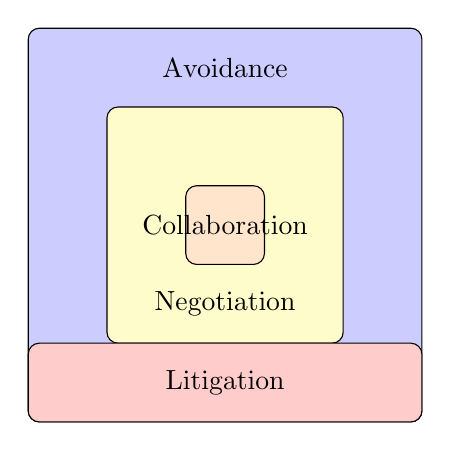
\begin{tikzpicture}
                    \draw[fill=blue!20, rounded corners] (0,0) rectangle (5,5);
                    \draw[fill=yellow!20, rounded corners] (1,1) rectangle (4,4);
                    \draw[fill=orange!20, rounded corners] (2,2) rectangle (3,3);
                    \draw[fill=red!20, rounded corners] (0,0) rectangle (5,1);
                    \node at (2.5,2.5) {Collaboration};
                    \node at (2.5,1.5) {Negotiation};
                    \node at (2.5,0.5) {Litigation};
                    \node at (2.5,4.5) {Avoidance};
                \end{tikzpicture}
                \caption{Conflict Resolution Pyramid}
            \end{figure}
            \end{frame}
            
            \begin{frame}
            \frametitle{Summary of Key Insights}
            \begin{itemize}
                \item \textbf{Conflict Sources:} Stakeholder interests, ideology, resources, regulations.
                \item \textbf{Conflict Management:} Negotiation, mediation, collaboration, litigation.
                \item \textbf{Opportunities:} Innovation, stakeholder engagement, stronger institutions.
            \end{itemize}
            
            \begin{figure}
                \centering
                \begin{tikzpicture}
                    \node[draw, circle, minimum size=2cm] (checklist) {\includegraphics[width=1.5cm]{checklist.png}};
                \end{tikzpicture}
                \caption{Key Takeaways}
            \end{figure}
            \end{frame}
            
            \begin{frame}
            \frametitle{Tips for Managing Policy Conflicts}
            \begin{itemize}
                \item Develop negotiation and mediation skills.
                \item Build trust and communication among stakeholders.
                \item Focus on flexibility and adaptive strategies.
                \item Prioritize evidence-based decision-making.
            \end{itemize}
            
            \begin{figure}
                \centering
                \begin{tikzpicture}
                    \node[draw, circle, minimum size=2cm] (handshake) {\includegraphics[width=1.5cm]{handshake.png}};
                    \node[draw, circle, minimum size=2cm, right of=handshake, xshift=3cm] (trust) {\includegraphics[width=1.5cm]{trust.png}};
                    \node[draw, circle, minimum size=2cm, right of=trust, xshift=3cm] (flexibility) {\includegraphics[width=1.5cm]{flexibility.png}};
                    \node[draw, circle, minimum size=2cm, right of=flexibility, xshift=3cm] (evidence) {\includegraphics[width=1.5cm]{research.png}};
                \end{tikzpicture}
                \caption{Tips for Managing Policy Conflicts}
            \end{figure}
            \end{frame}
            
            \begin{frame}
            \frametitle{Reflecting on Policy Conflict}
            \begin{itemize}
                \item How can understanding conflict improve your role as a policymaker?
                \item What strategies will you apply in your own policy work?
                \item Can conflict management turn challenges into opportunities?
            \end{itemize}
            
            \begin{figure}
                \centering
                \begin{tikzpicture}
                    \node[draw, circle, minimum size=2cm] (reflection) {\includegraphics[width=1.5cm]{reflection.png}};
                \end{tikzpicture}
                \caption{Reflecting on Policy Conflicts}
            \end{figure}
            \end{frame}
            
            \begin{frame}
            \frametitle{Looking Ahead}
            \begin{itemize}
                \item \textbf{Summary:}
                    \begin{itemize}
                        \item Conflict is inherent to policymaking.
                        \item Effective management can lead to better outcomes.
                    \end{itemize}
                \item \textbf{Next Week's Topic:} Public Policy Implementation.
            \end{itemize}
            
            \begin{figure}
                \centering
                \includegraphics[width=0.6\textwidth]{path-forward.png}
                \caption{Progressing to Policy Implementation}
            \end{figure}
            \end{frame}

\end{document}
